\documentclass[aps, prl, reprint, groupedaddress]{revtex4-1}

\usepackage{physics}
\usepackage{graphicx}
\usepackage{subfig}
\usepackage{multirow}
\usepackage{bm}

\begin{document}
    
\title{Monte Carlo methods for Solving PDEs\\- Report for Computational Physics Final Project}
\author{Yucheng Zhang}
\email{yz4035@nyu.edu}
\affiliation{Department of Physics, New York University}
\date{\today}
    
\begin{abstract}
    This is the report for the Computational Physics final project.
\end{abstract}
    
\maketitle

\section{Introduction}

There are many numerical methods for solving different types of Partial Differential Equations (PDEs) in Boundary Value Problems (BVPs), such as the relaxation method and the Gauss-Seidel method. These methods are all deterministic methods. In this report, we explore the Monte Carlo method for solving PDEs in BVPs. 

We mainly focus on Laplace's Equation with Dirichlet Boundary Conditions,
\begin{equation}
    \nabla^2 u = 0
    \label{eq:laplace}
\end{equation} inside the boundary, and
\begin{equation}
    u = f(x)
\end{equation} on the boundary. In 2D, the Laplace's Equation Eq.~\ref{eq:laplace} can be discreted with finite difference approximation, the centered difference reads,
\begin{equation}
    u_{i,j} = \frac{1}{4} \qty(u_{i+1,j}+u_{i-1,j}+u_{i,j+1}+u_{i,j-1}).
\end{equation}
As shown in FIG.~\ref{fig:disc}.

\begin{figure}[htbp]
    \centering
    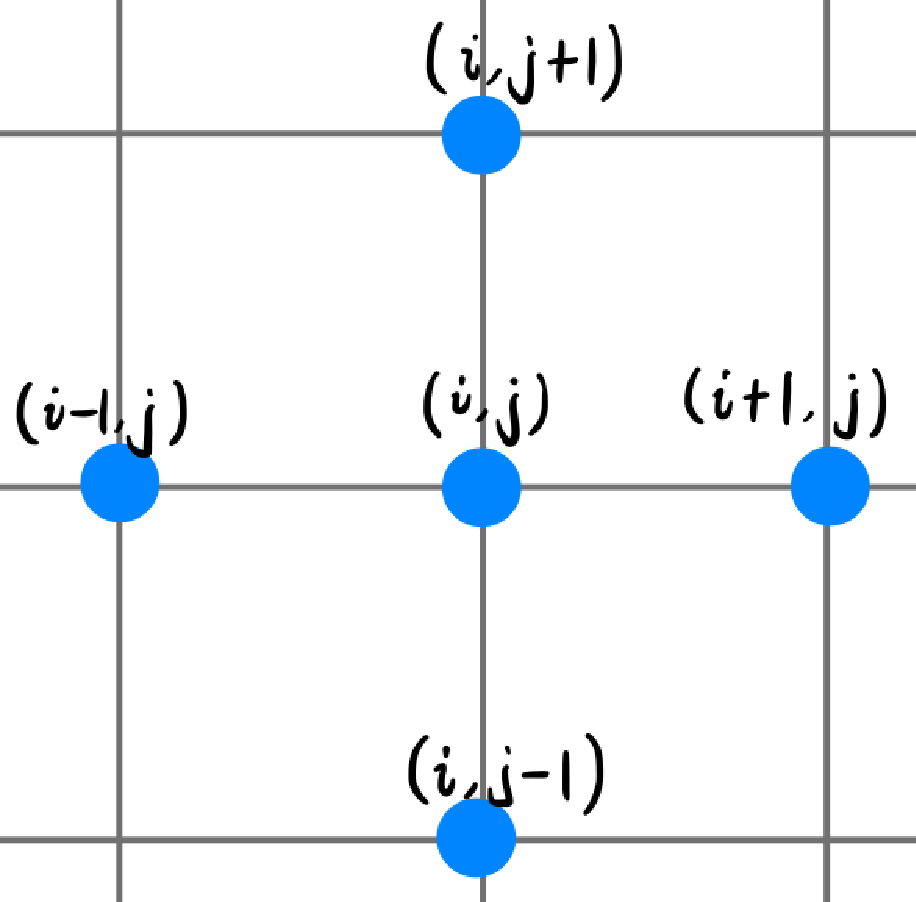
\includegraphics[width=.4\textwidth]{./figs/disc}
    \caption{\label{fig:disc} Finite centered difference on 2D.}
\end{figure}

For the relaxation method, we use this equation, start from the boundary, and iterate until we get the desired accuracy. Here we look at this equation in a different way. We should notice that the value at one point is the average of its neighbours' values. So we can regard the $\frac{1}{4}$ as the statistical weight of each neighbour while calculating the value of the center point. Then we can construct the Monte Carlo method based on this point of view.

\subsection{Simple Random Walk Method}

\begin{figure}[htbp]
    \centering
    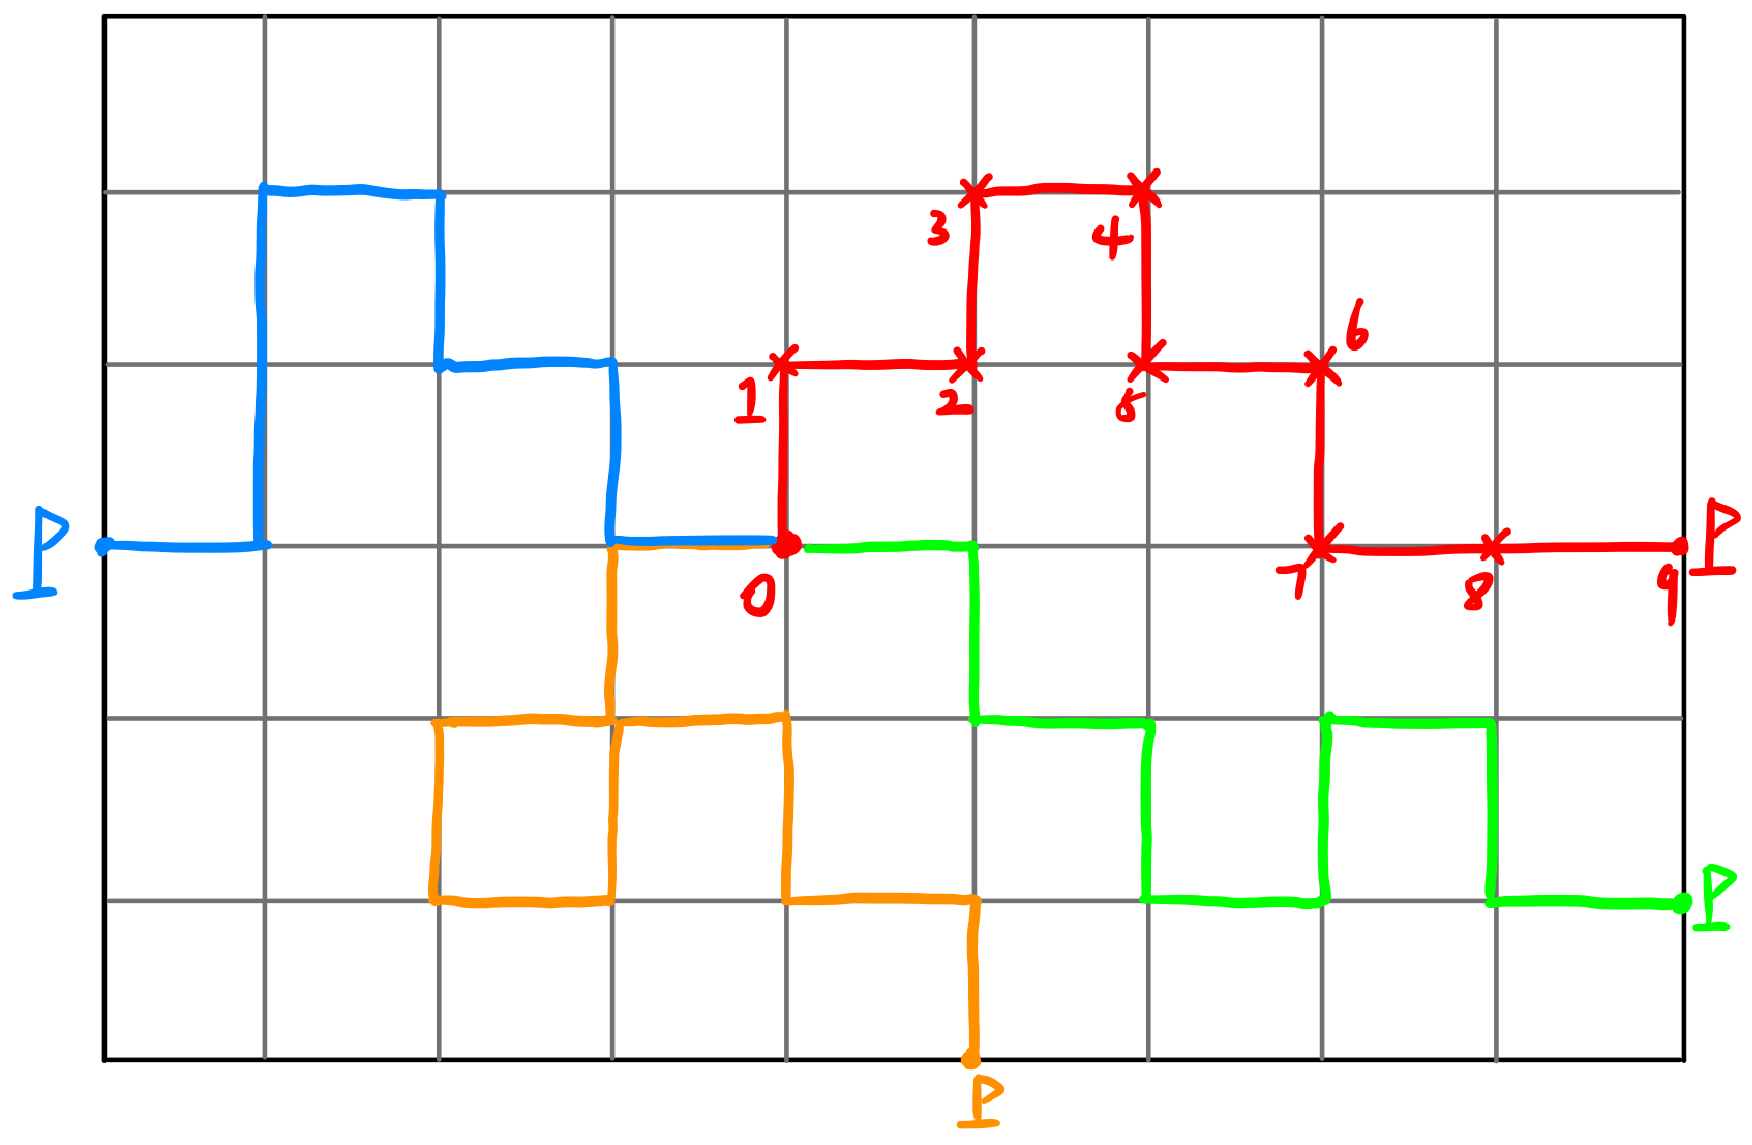
\includegraphics[width=.4\textwidth]{./figs/srw}
    \caption{\label{fig:srw} Simple Random Walk method.}
\end{figure}

Given the point $P_0$ whose value we want to evaluate on the grid,
\begin{enumerate}
    \item Pick a neighbour point, e.g. $P_1$, with proper probability randomly, here it's $\frac{1}{4}$ for each point.
    \item We don't know the value at $P_1$, but we know it's the average of its neighbours, so pick one of it's neighbours, e.g. $P_2$. Continue this process, until we reach a point on the boundary, e.g. $P_n$, whose value is given.
    \item We know that $P_n$ is an estimate of $P_{n-1}$, which is an estimate of $P_{n-2}$, etc, etc, all the way back to $P_0$. So after this random walk process, we get an estimate of $P_0$.
    \item Do a large amount of random walks from $P_0$ to the boundary, then average all the estimates, we can get a good estimate of the value at $P_0$, whose accuracy depends on the number of random walks, i.e. the number of estimates.
\end{enumerate}

% Poisson equation

\subsection{Walk on Spheres}

As we should notice, for the Laplace Equation, one estimate given by one random walk is just the value at the point on the boundary where the random walk ends. So the estimate doesn't depend on the path of the random walk. If we let the grid spacing go to zero, which obviously will increase the accuracy of the estimate, then the random walk here becomes simple Brownian motion.

Consider a sphere centered at $\bm{r}$, for a simple Brownian motion starting from $\bm{r}$, the possibility for the motion to reach any point on the sphere is equal. So since the path doesn't matter here for the Laplace equation, why do we simulate the Brownian motion step by step? We can jump to one point on the sphere directly!

\begin{figure}[htbp]
    \centering
    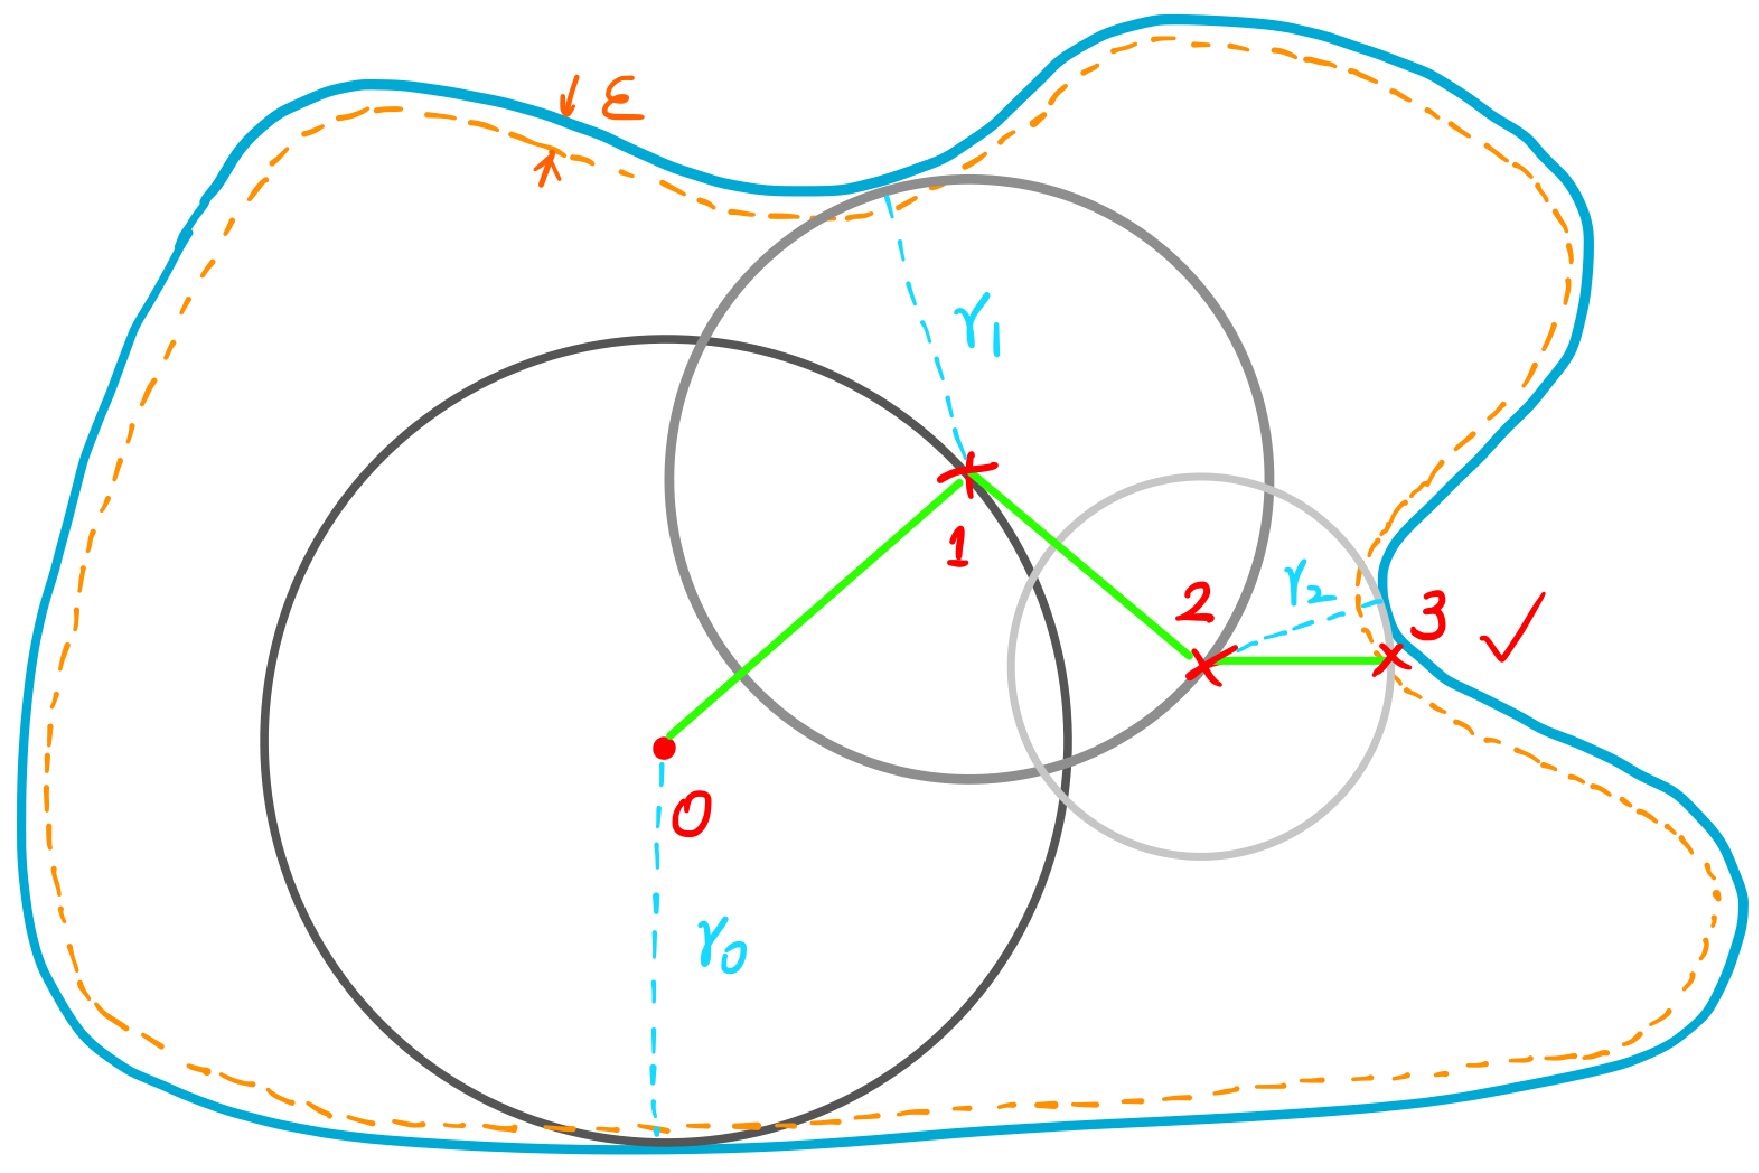
\includegraphics[width=.46\textwidth]{./figs/wos}
    \caption{\label{fig:wos} Walk on Spheres method.}
\end{figure}

The Walk on Spheres (WoS) method is shown in FIG.~\ref{fig:wos}. Here are some explainations.
\begin{itemize}
    \item The radius of the spheres (circles in 2D) are determined by the shortest distance from the point to the boundary, e.g. $r_0$, $r_1$, and $r_2$ in FIG.~\ref{fig:wos}.
    \item The next point is chosen randomly on the sphere, e.g. points $1, 2, 3$ in FIG.~\ref{fig:wos}.
    \item Since the WoS method is grid-free, we use the shell with thickness $\epsilon$ to judge whether the random motion reaches the boundary, as shown in FIG.~\ref{fig:wos}.
\end{itemize}


\subsection{Characteristics of Monte Carlo method}

Both the Simple Random Walk (SRW) and Walk on Spheres (WoS) methods are Monte Carlo methods. The Monte Carlo methods here have some characteristics and advantages that normal deterministic methods don't have.

\subsubsection{Independence of points}

The first thing to notice is that unlike the relaxation or Gauss-Seidel methods, the points on the grid for the SRW or on the grid-free WoS, they are all independent. So it's very fast to estimate some point values.

\subsubsection{Boundary \& Dimension}

For the Monte Carlo methods here, the boundary doesn't matter a lot. The only thing is to decide whether the random walk reaches the boundary, and at which point. So it's relatively easy for these methods to handle some problems with complex boundaries. Also, it's easier for these methods to be extended to higher dimensions.

\subsubsection{Parallel Computing}

Not only different points, as mentioned above, but also different estimates for one point are independent. So these Monte Carlo methods are naturally parallel. The two most straightforward ways to parallelize the program are,
\begin{itemize}
    \item Parallelize the different estimates of one point, then average the results from different processes.
    \item Parallelize the set of points to be evaluated.
\end{itemize}


\section{Implementation \& Analysis}

In this section, we first introduce how the programs are implemented. Then we use these methods to study two practical problems and analyze the properties of these methods.

\subsection{Parallelization in \emph{Python}}

In \emph{Python}, there are many packages for parallel computing. In this project, we use the \emph{multiprocessing} package. For a given set of points to be evaluated, we allocate the total number of independent estimates of every point to all available cores. Then we initialize the random number generators in all processes with different seeds. Here we use the \emph{numpy.random} module to produce random numbers, which can be initialized with \emph{numpy.random.RandomState(seed)}.

\subsection{Square Boundary Problem}

Assume we have a 2D Laplace problem with the boundary given as a square.

\begin{figure}[htbp]
    \centering
    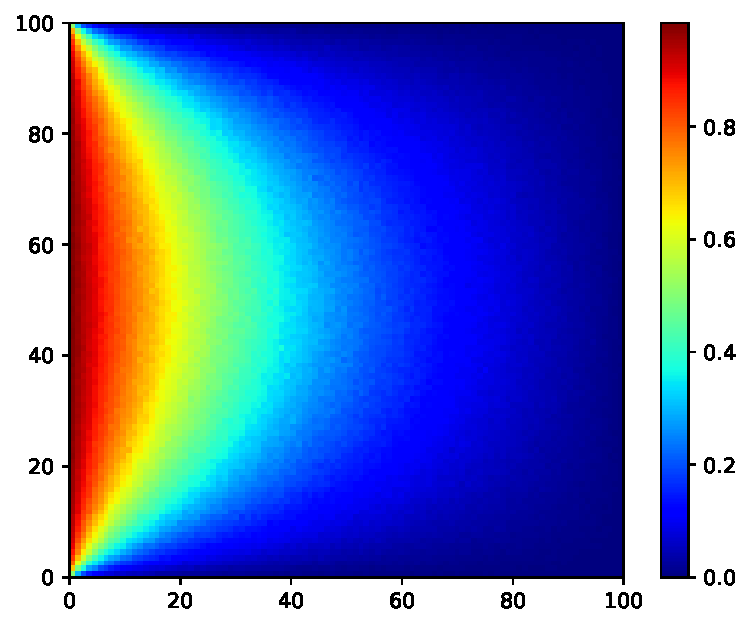
\includegraphics[width=.4\textwidth]{./figs/srw_s}
    \caption{\label{fig:srw_s} SRW method on 2D Square Boundary with Square Lattice.}
\end{figure}

\begin{figure}[htbp]
    \centering
    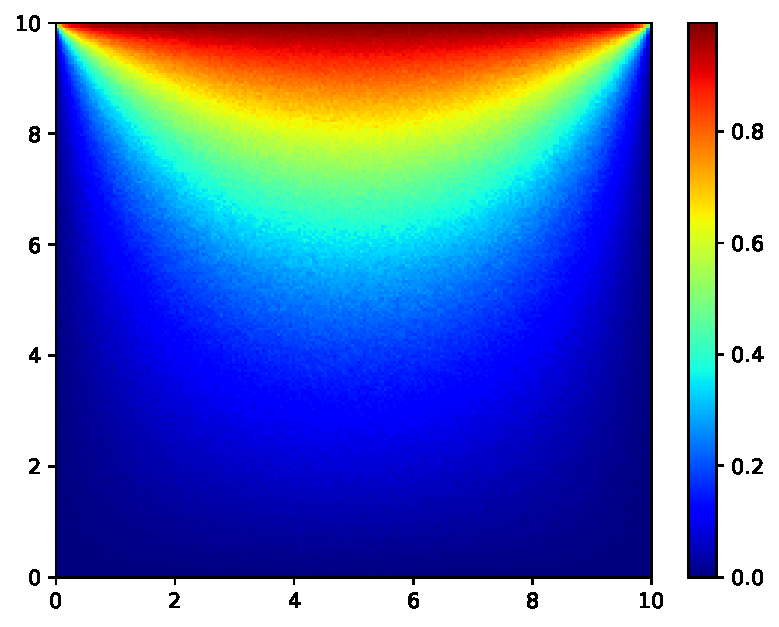
\includegraphics[width=.4\textwidth]{./figs/wos_s}
    \caption{\label{fig:wos_s} WoS method on 2D Square Boundary.}
\end{figure}

\subsection{Circle Boundary Problem}

Here we study the 2D Laplace problem with a circle boundary.

\begin{figure}[htbp]
    \centering
    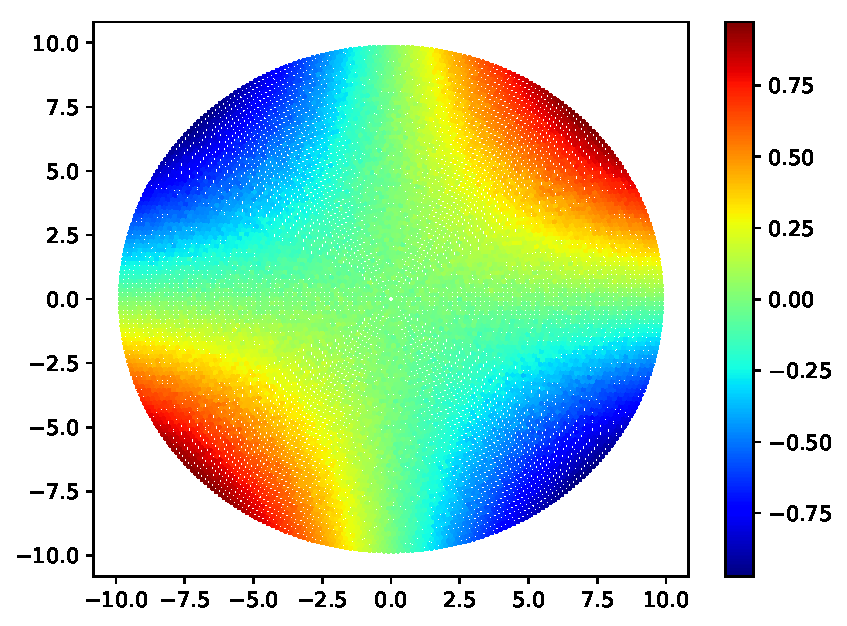
\includegraphics[width=.4\textwidth]{./figs/wos_c}
    \caption{\label{fig:wos_c} WoS method on 2D Circle Boundary.}
\end{figure}

\subsection{The Influence of $\epsilon$}

\begin{figure}[htbp]
    \centering
    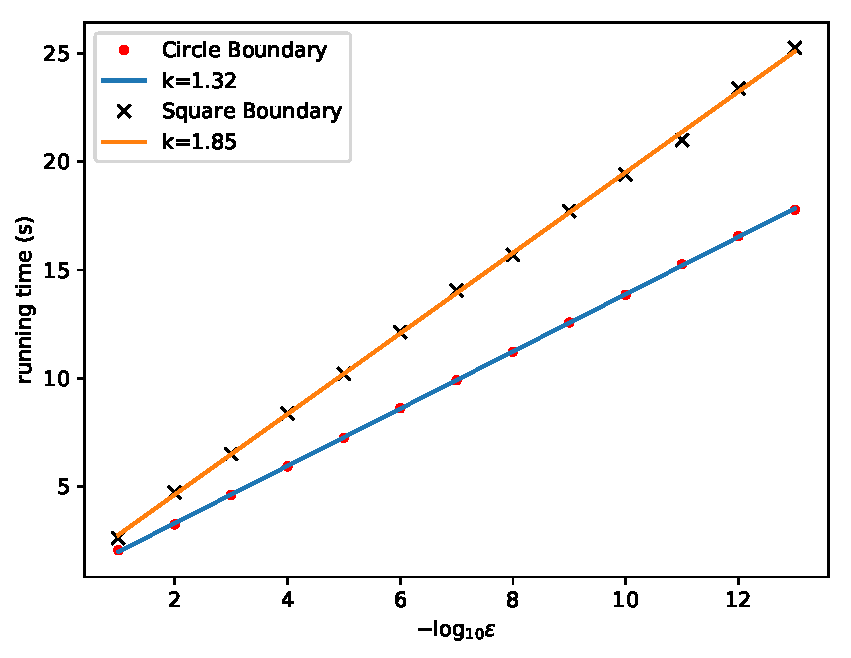
\includegraphics[width=.4\textwidth]{./figs/ep_t}
    \caption{\label{fig:ep_t} The running time - $\epsilon$ relation on both square and circle boundary.}
\end{figure}

\section{Summary \& Future Work}



\section{Acknowledgement}

\bibliography{}

\end{document}
